\documentclass{article}

\usepackage{cmcphys}
\usepackage[margin=1.0in]{geometry}
\usepackage[titletoc,title]{appendix}
\allowdisplaybreaks

\graphicspath{{figures/}}

\renewcommand{\L}{\mathcal{L}}
\newcommand{\e}{\mathrm{e}}
\renewcommand{\i}{\mathrm{i}}
\renewcommand{\Re}{\mathrm{Re}\ }

\title{Chaotic Behavior of the Triple Pendulum \\
    \large A Computational Approach }
\author{Rachel Bass \and Cory McCartan}
\date{May 2017}

\begin{document}

\maketitle

\section{Introduction}
In this paper, we will report on our findings regarding the behavior and
motion of an undamped triple pendulum made of three equal masses attached by
three massless rods of equal length. We used the Lagrangian formulation to
create equations of motion for the three masses, then examined the system using
Python. We used Fourier transformations as a tool to help us determine if the
pendulum's motion was chaotic or periodic. \textbf{Did we examine how changing
the masses affects the motion or are we giving up on that?} Our findings helped
us find some order about a system that initially appeared to be purely chaotic.
    
\section{Conservation of Energy}
After finding our equations of motion for the three masses, we first wanted to
test that they were correct. Our plots of the masses' angles versus time seemed
reasonable, but we wanted to confirm our suspicions before delving deeper into
the problem. We plotted kinetic, potential and total energy versus time on the
same set of axes and saw that mechanical energy of the system is conserved
(Fig. \ref{fig:energy_cons}).
\begin{figure}[h]
	\centering
	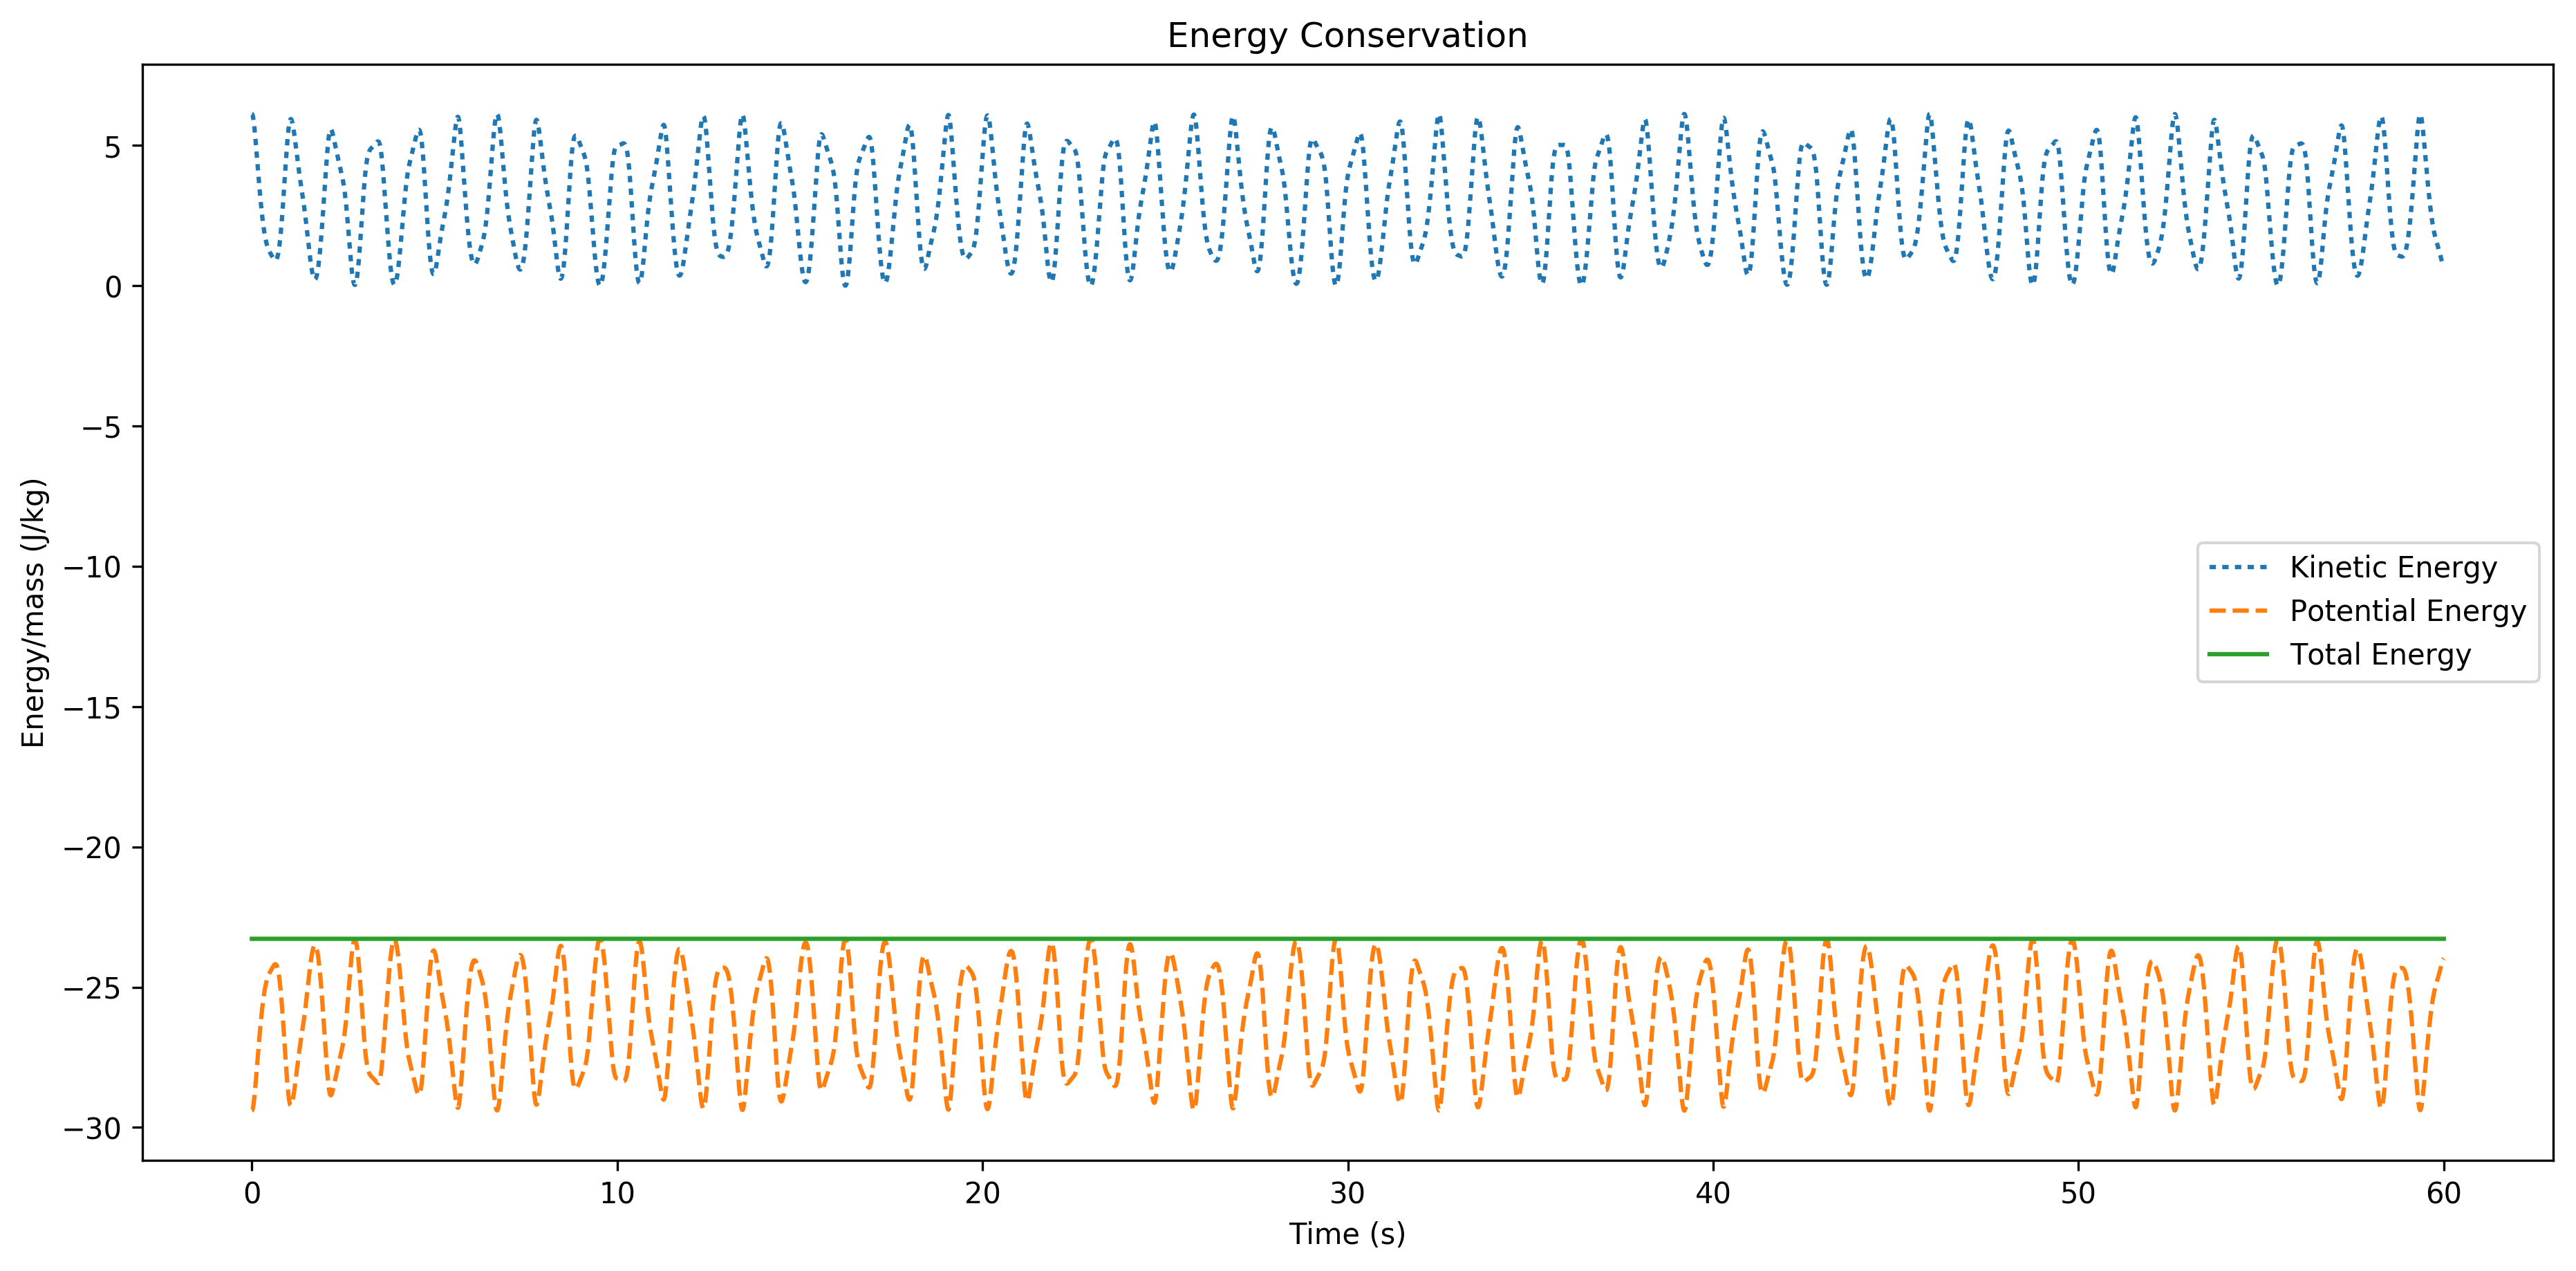
\includegraphics[width=\textwidth]{energy_conservation}
	\caption{Kinetic, potential, and total energy over time for $\dot\phi_3(0)=\SI{7}{s^{-1}}$.}
	\label{fig:energy_cons}
\end{figure}

\section{Chaotic or Periodic?}
As we first began to examine the system, we kept all initial angles and angular
velocities save for the lowest hanging mass's at zero. For short time frames
and an initial angular velocity of $\dot\phi_3=\SI{7}{s^{-1}}$, the motion of
the system appears to be chaotic. However, increasing the time window to 1,000
seconds showed something different. In Figure \ref{fig:moderate_time}, we can
see that there appears to be some sort of regularity to the pendulum's motion.
Looking at such a plot is not sufficient to declare periodic victory, so we
needed to use some other tools to help us describe the system's motion.
 \begin{figure}
	\centering
	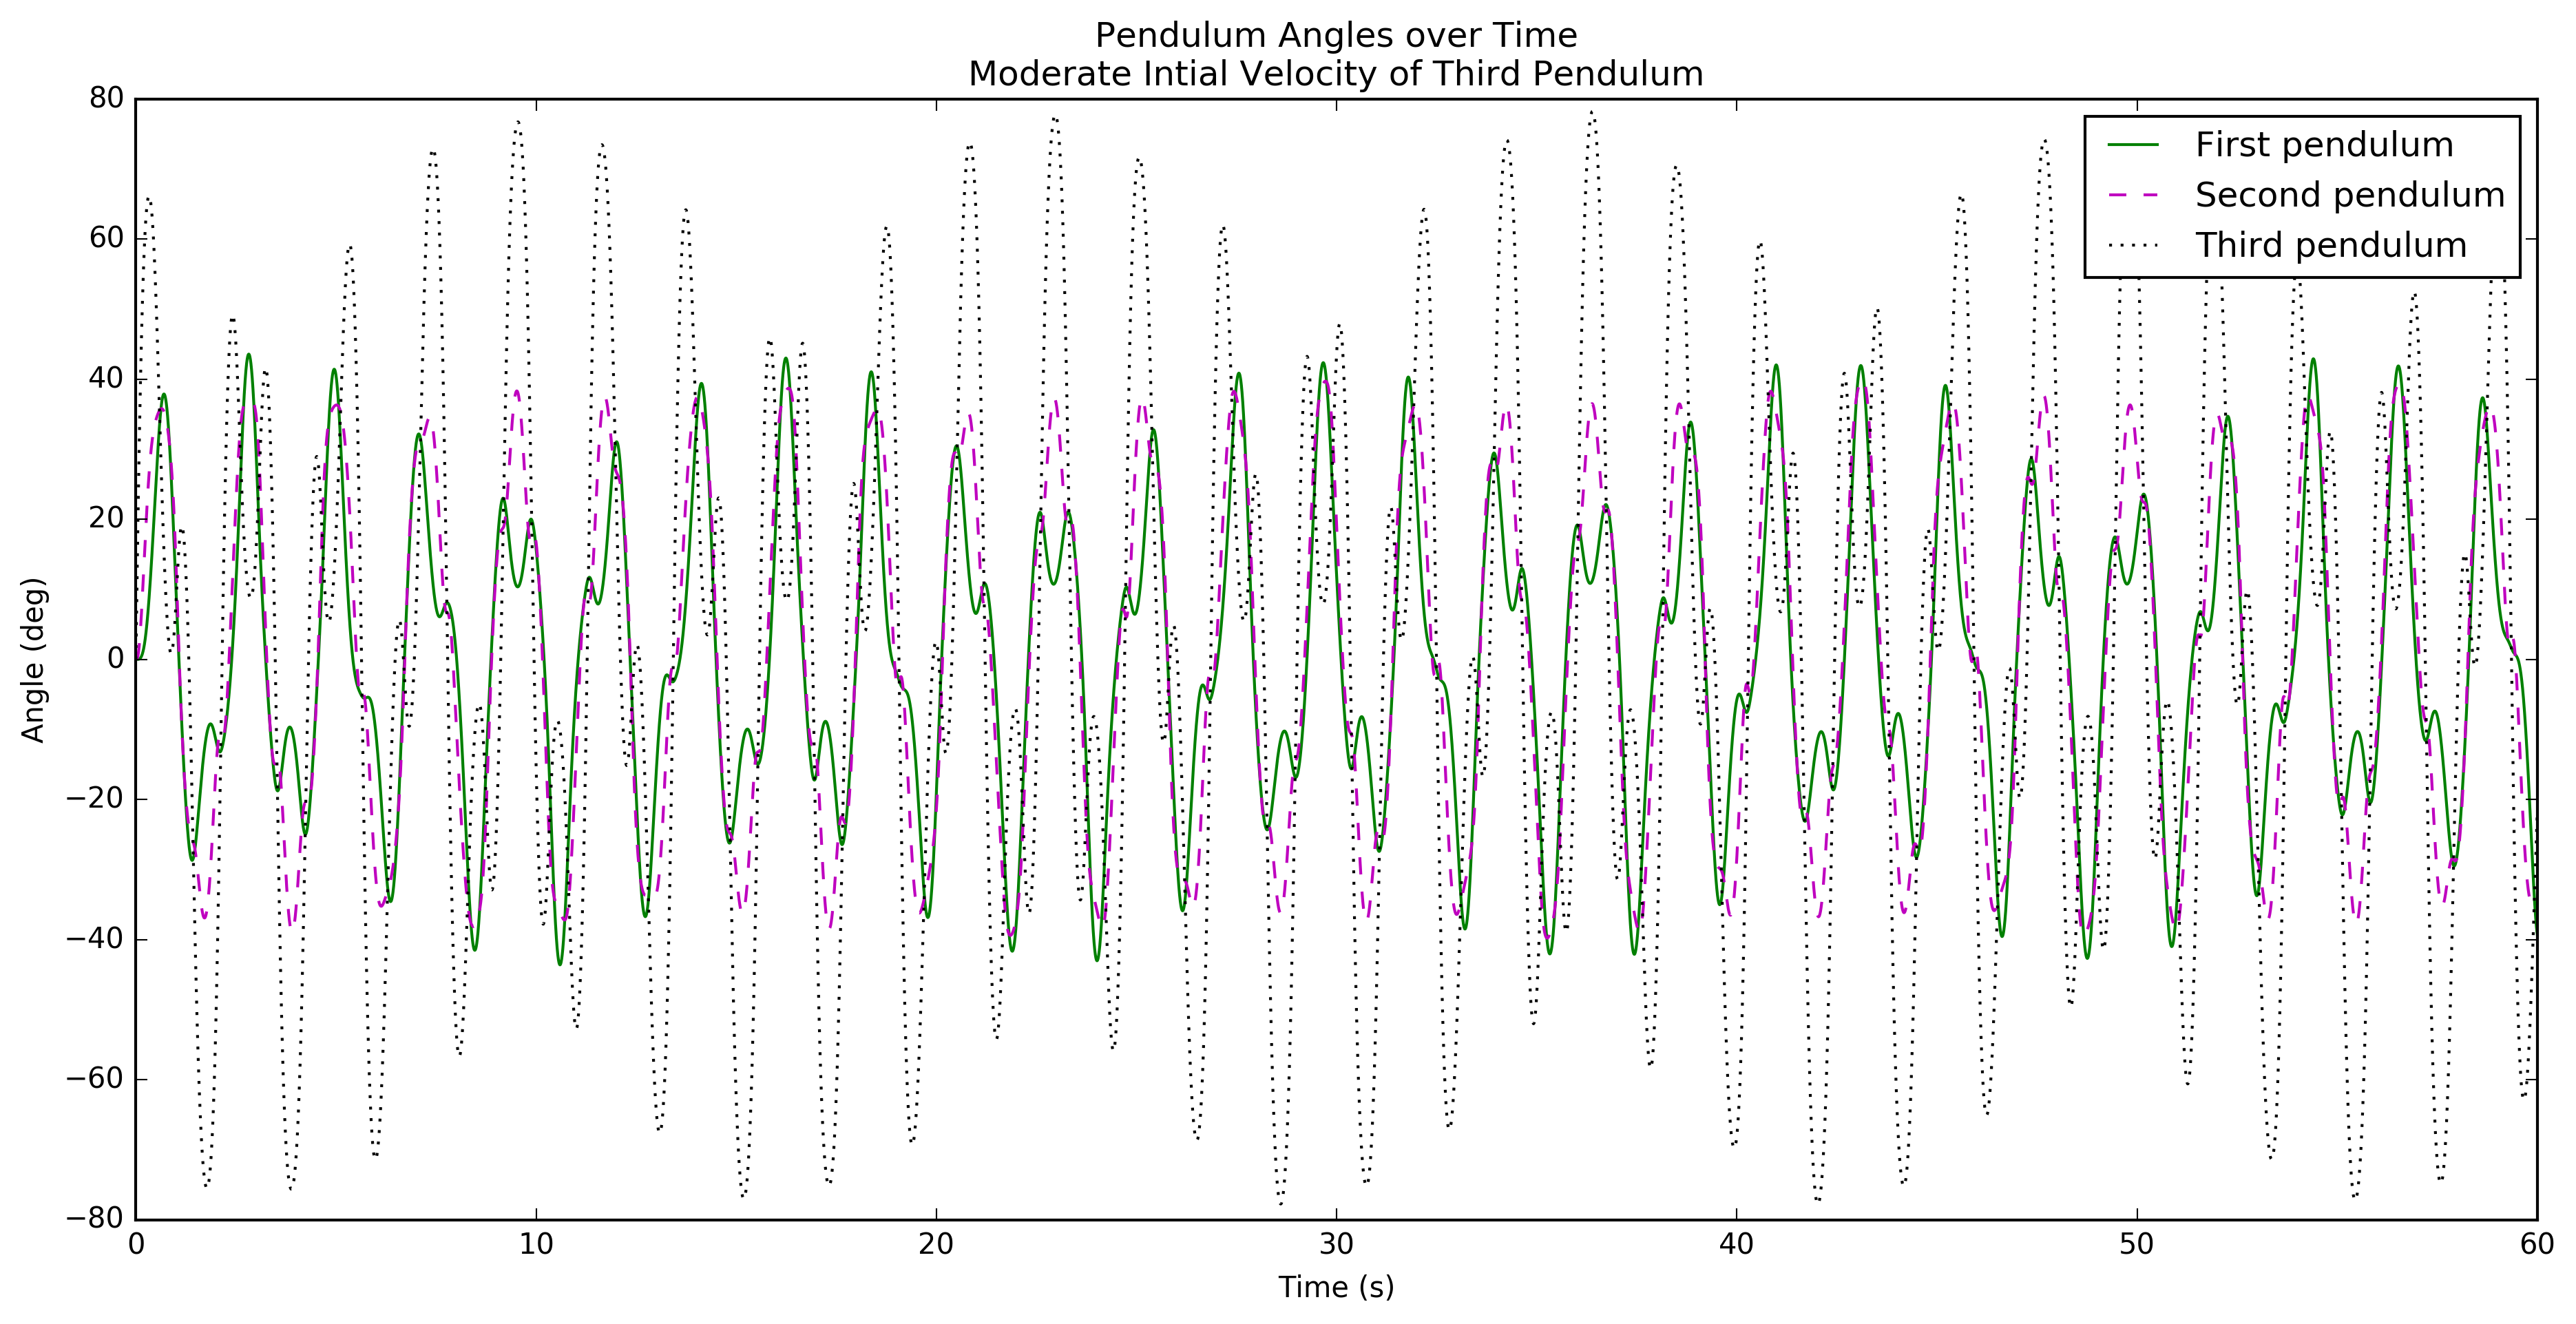
\includegraphics[width=\textwidth]{moderate_velocity_time_sol}
	\caption{$\phi_1,\phi_2$, and $\phi_3$ over time for $\dot\phi_3(0)=\SI{7}{s^{-1}}$}
	\label{fig:moderate_time}
\end{figure}

\section{Results}

\begin{figure}
	\centering
	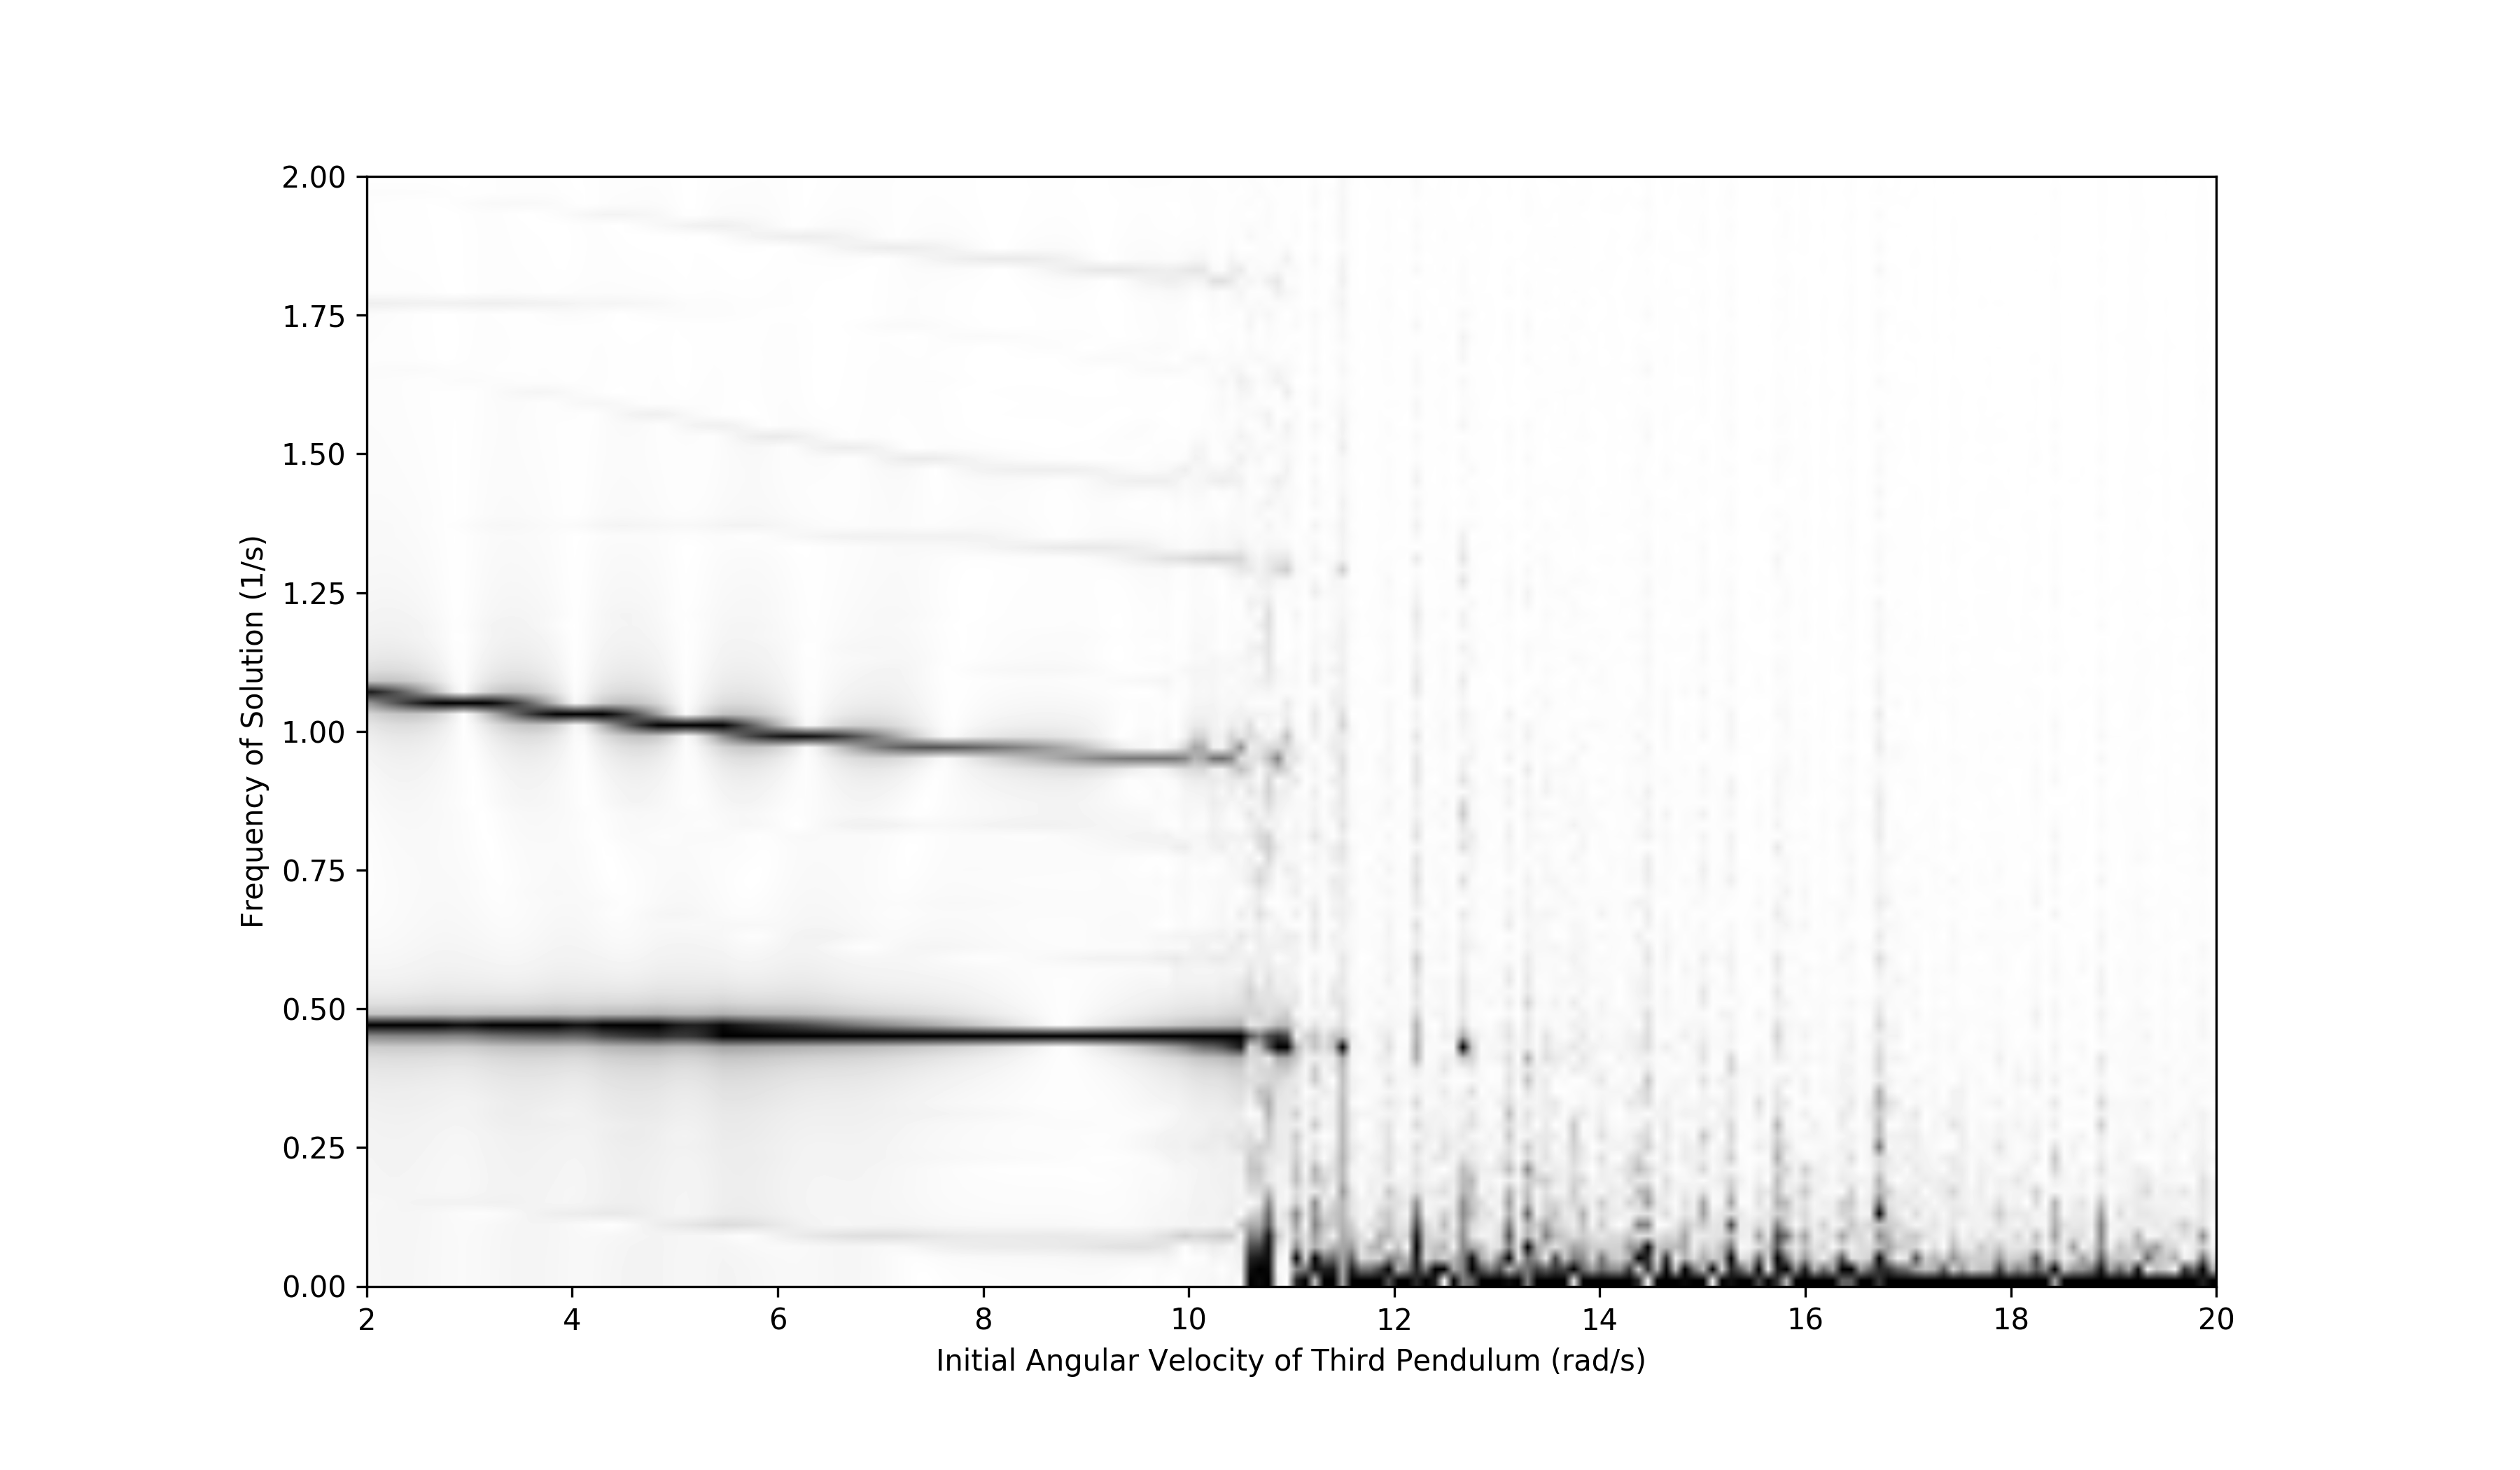
\includegraphics[width=\textwidth]{bifurcation_1}
	\caption{``Bifurcation Diagram" for $2\le\dot\phi_3(0)\le 20$}
	\label{fig:bifurc_1}
\end{figure}

\clearpage
\begin{appendices}

\section{Equations of Motion}

\begin{wrapfigure}[13]{r}{0.25\textwidth}
	\centering
	\includegraphics[width=0.2\textwidth]{drawing.tikz}
	\caption{The triple pendulum.}
\end{wrapfigure}

We can describe the position of a given mass by its Cartesian coordinates
$(x_i, y_i)$.  The position of a given mass is the sum of its position
relative to its pivot point and the position of its pivot point:
\begin{align}
	x_1 &= l\sin\phi_1     & y_1 &= -l\cos\phi_1 \\
	x_2 &= x_1+l\sin\phi_2 & y_2 &= y_1 + -l\cos\phi_2 \\
	x_3 &= x_2+l\sin\phi_3 & y_3 &= y_2 + -l\cos\phi_3.
\end{align}
Making the appropriate substitutions, we have
\begin{align}
	x_1 &= l\sin\phi_1     \\
	y_1 &= -l\cos\phi_1 \\
	x_2 &= l(\sin\phi_1+\sin\phi_2)  \\
	y_2 &= -l(\cos\phi_1+\cos\phi_2) \\
	x_3 &= l(\sin\phi_1+\sin\phi_2+\sin\phi_3)  \\
	y_3 &= -l(\cos\phi_1+\cos\phi_2+\cos\phi_3).
\end{align}
Taking time derivatives to find velocity, we have
\begin{align}
	\dot x_1 &= l\dot\phi_1\cos\phi_1 \\
	\dot y_1 &= l\dot\phi_1\sin\phi_1 \\
	\dot x_2 &= l(\dot\phi_1\cos\phi_1+\dot\phi_2\cos\phi_2) \\
	\dot y_2 &= l(\dot\phi_1\sin\phi_1+\dot\phi_2\sin\phi_2) \\
	\dot x_3 &= l(\dot\phi_1\cos\phi_1+\dot\phi_2\cos\phi_2
		+\dot\phi_3\cos\phi_3) \\
	\dot y_3 &= l(\dot\phi_1\sin\phi_1+\dot\phi_2\sin\phi_2
		+\dot\phi_3\sin\phi_3).
\end{align}
For the kinetic energy, we will need to find $v^2={\dot x}^2{\dot y}^2$ for
each mass. 
\begin{align}
	v_1^2 &= {\dot x_1}^2+{\dot y_1}^2 \\
	&= (l\dot\phi_1\cos\phi_1)^2
		+(l\dot\phi_1\sin\phi_1)^2 \\
	&= l^2(\dot\phi_1^2\cos^2\phi_1+\dot\phi_1^2\sin^2\phi_1) \\
	&= l^2\dot\phi_1^2 \\\\
			%
	v_2^2 &= {\dot x_2}^2+{\dot y_2}^2 \\
	&= (l(\dot\phi_1\cos\phi_1+\dot\phi_2\cos\phi_2))^2
	  +(l(\dot\phi_1\sin\phi_1+\dot\phi_2\sin\phi_2))^2 \\
	&= l^2\left( \dot\phi_1^2\cos^2\phi_1 
		+ 2\dot\phi_1\dot\phi_2\cos\phi_1\cos\phi_2 
		+ \dot\phi_2^2\cos^2\phi_2 + \dot\phi_1^2\sin^2\phi_1 
		+ 2\dot\phi_1\dot\phi_2\sin\phi_1\sin\phi_2 
		+ \dot\phi_2^2\sin^2\phi_2 \right) \\
	&= l^2\left( \dot\phi_1^2\cos^2\phi_1 + \dot\phi_1^2\sin^2\phi_1
		+ \dot\phi_2^2\cos^2\phi_2 + \dot\phi_2^2\sin^2\phi_2
		+ 2\dot\phi_1\dot\phi_2(\cos\phi_1\cos\phi_2 + \sin\phi_1\sin\phi_2)
		 \right) \\
	&= l^2\left( \dot\phi_1^2 + \dot\phi_2^2
		+ 2\dot\phi_1\dot\phi_2\cos(\phi_1 - \phi_2) \right) \\\\
			%
	v_3^2 &= {\dot x_3}^2+{\dot y_3}^2 \\
	&= (l(\dot\phi_1\cos\phi_1+\dot\phi_2\cos\phi_2+\dot\phi_3\cos\phi_3))^2 
	  +(l(\dot\phi_1\sin\phi_1+\dot\phi_2\sin\phi_2+\dot\phi_3\sin\phi_3))^2 \\
	&= l^2\bigl( \dot\phi_1^2\sin^2\phi_1+\dot\phi_2^2\sin^2\phi_2
	   +\dot\phi_3^2\sin^2\phi_3 + 2\dot\phi_1\dot\phi_2\sin\phi_1\sin\phi_2
	   +2\dot\phi_1\dot\phi_3\sin\phi_1\sin\phi_3
	   +2\dot\phi_2\dot\phi_3\sin\phi_2\sin\phi_3 \\
	   &\quad +\dot\phi_1^2\cos^2\phi_1+\dot\phi_2^2\cos^2\phi_2
	   +\dot\phi_3^2\cos^2\phi_3 + 2\dot\phi_1\dot\phi_2\cos\phi_1\cos\phi_2
	   +2\dot\phi_1\dot\phi_3\cos\phi_1\cos\phi_3
	   +2\dot\phi_2\dot\phi_3\cos\phi_2\cos\phi_3
	\bigr) \\
	&= l^2\left( \dot\phi_1^2+\dot\phi_2^2 +\dot\phi_3^2 
	   +2\dot\phi_1\dot\phi_2\cos(\phi_1-\phi_2)
	   +2\dot\phi_1\dot\phi_3\cos(\phi_1-\phi_3)
	   +2\dot\phi_2\dot\phi_3\cos(\phi_2-\phi_3) \right) 
\end{align}
We can now write the kinetic and potential energy for the system by summing
up $-mgy_i$ and $\frac{1}{2}mv_i^2$ for each mass $i$:
\begin{align}
	U &= U_1 + U_2 + U_3 \\
	&= -mgl\left(3\cos\phi_1+2\cos\phi_2+\cos\phi_3 \right) \\\\
			%
	T &= T_1 + T_2 + T_3 \\
	&= \frac{1}{2}ml^2 \left( 3\dot\phi_1^2+2\dot\phi_2^2+\dot\phi_3^2
	   + 4\dot\phi_1\dot\phi_2\cos(\phi_1-\phi_2)
	   + 2\dot\phi_1\dot\phi_3\cos(\phi_1-\phi_3)
	   + 2\dot\phi_2\dot\phi_3\cos(\phi_2-\phi_3) \right) 
\end{align}
So the Lagrangian is
\begin{align}
	\L &= T - U \\
	&= mgl\left(3\cos\phi_1+2\cos\phi_2+\cos\phi_3 \right) 
	   + \frac{1}{2}ml^2 \bigl( 3\dot\phi_1^2+2\dot\phi_2^2+\dot\phi_3^2
	   + 4\dot\phi_1\dot\phi_2\cos(\phi_1-\phi_2) \\
	&\qquad\qquad + 2\dot\phi_1\dot\phi_3\cos(\phi_1-\phi_3)
	   + 2\dot\phi_2\dot\phi_3\cos(\phi_2-\phi_3) \bigr) 
\end{align}
Since our generalized coordinates are $\phi_1,\phi_2$, and $\phi_3$, we must
now take partial derivatives of the Lagrangian with respect to each $\phi_i$
and $\dot\phi_i$:
\begin{align}
	\pD{\L}{\phi_1} &= -3mgl\sin\phi_1 
		-2ml^2\dot\phi_1\dot\phi_2\sin(\phi_1-\phi_2)
		-ml^2\dot\phi_1\dot\phi_3\sin(\phi_1-\phi_3) \\
	\pD{\L}{\phi_2} &= -2mgl\sin\phi_2 
		+2ml^2\dot\phi_1\dot\phi_2\sin(\phi_1-\phi_2)
		-ml^2\dot\phi_2\dot\phi_3\sin(\phi_2-\phi_3) \\
	\pD{\L}{\phi_3} &= -mgl\sin\phi_3 
		+ml^2\dot\phi_1\dot\phi_3\sin(\phi_1-\phi_3)
		+ml^2\dot\phi_2\dot\phi_3\sin(\phi_2-\phi_3) \\\\
			%
	\pD{\L}{\dot\phi_1} &= 3ml^2\dot\phi_1 
		+ 2ml^2\dot\phi_2\cos(\phi_1-\phi_2) 
		+ ml^2\dot\phi_3\cos(\phi_1-\phi_3)  \\
	\pD{\L}{\dot\phi_2} &= 2ml^2\dot\phi_2 
		+ 2ml^2\dot\phi_1\cos(\phi_1-\phi_2) 
		+ ml^2\dot\phi_3\cos(\phi_2-\phi_3)  \\
	\pD{\L}{\dot\phi_3} &= ml^2\dot\phi_3 
		+ ml^2\dot\phi_1\cos(\phi_1-\phi_3) 
		+ ml^2\dot\phi_2\cos(\phi_2-\phi_3) 
\end{align}
Next, we find $\D{}{t}\pD{\L}{\dot\phi_i}$ for each $i$:
\begin{align}
	\D{}{t}\pD{\L}{\dot\phi_1} &= 3ml^2\ddot\phi_1 
		+ 2ml^2\ddot\phi_2\cos(\phi_1-\phi_2) 
		- 2ml^2\dot\phi_2\sin(\phi_1-\phi_2)(\dot\phi_1-\dot\phi_2) \\
		&\quad + ml^2\ddot\phi_3\cos(\phi_1-\phi_3) 
		- ml^2\dot\phi_3\sin(\phi_1-\phi_3)(\dot\phi_1-\dot\phi_3) \\\\
	\D{}{t}\pD{\L}{\dot\phi_2} &= 2ml^2\ddot\phi_2 
		+ 2ml^2\ddot\phi_1\cos(\phi_1-\phi_2) 
		- 2ml^2\dot\phi_1\sin(\phi_1-\phi_2)(\dot\phi_1-\dot\phi_2) \\
		&\quad + ml^2\ddot\phi_3\cos(\phi_2-\phi_3) 
		- ml^2\dot\phi_3\sin(\phi_2-\phi_3)(\dot\phi_2-\dot\phi_3) \\\\
	\D{}{t}\pD{\L}{\dot\phi_3} &= ml^2\ddot\phi_3 
		+ ml^2\ddot\phi_1\cos(\phi_1-\phi_3) 
		- ml^2\dot\phi_1\sin(\phi_1-\phi_3)(\dot\phi_1-\dot\phi_3) \\
		&\quad + ml^2\ddot\phi_2\cos(\phi_2-\phi_3) 
		- ml^2\dot\phi_2\sin(\phi_2-\phi_3)(\dot\phi_2-\dot\phi_3) 
\end{align}
We can then write the equations of motion for each of our generalized
coordinates, according to the Euler-Lagrange condition $\pD{\L}{\phi_i}
=\D{}{t}\pD{\L}{\dot\phi_i}$. For $\phi_1$ we have
\begin{align}
	\pD{\L}{\phi_1} &= \D{}{t}\pD{\L}{\dot\phi_1} 
\end{align}
\begin{align}
	-3mgl\sin\phi_1 -2ml^2\dot\phi_1\dot\phi_2\sin(\phi_1-\phi_2)
		-ml^2\dot\phi_1\dot\phi_3\sin(\phi_1-\phi_3)
	&= 3ml^2\ddot\phi_1 + 2ml^2\ddot\phi_2\cos(\phi_1-\phi_2) \\
	&\quad - 2ml^2\dot\phi_2\sin(\phi_1-\phi_2)(\dot\phi_1-\dot\phi_2) \\
	&\quad + ml^2\ddot\phi_3\cos(\phi_1-\phi_3) \\
	&\quad - ml^2\dot\phi_3\sin(\phi_1-\phi_3)(\dot\phi_1-\dot\phi_3) 
\end{align}
\begin{align}
	-3mgl\sin\phi_1 &= 3ml^2\ddot\phi_1 + 2ml^2\ddot\phi_2\cos(\phi_1-\phi_2)
		+ ml^2\ddot\phi_3\cos(\phi_1-\phi_3)  \\
		&\quad + 2ml^2\dot\phi_2^2\sin(\phi_1-\phi_2)
		+ ml^2\dot\phi_3^2\sin(\phi_1-\phi_3)
\end{align}
\begin{align}
	-\frac{3g}{l}\sin\phi_1 &= 3\ddot\phi_1 + 2\ddot\phi_2\cos(\phi_1-\phi_2)
		+ \ddot\phi_3\cos(\phi_1-\phi_3) + 2\dot\phi_2^2\sin(\phi_1-\phi_2)
		+ \dot\phi_3^2\sin(\phi_1-\phi_3)   \label{eq_m1}
\end{align}

For $\phi_2$ we have
\begin{align}
	\pD{\L}{\phi_2} &= \D{}{t}\pD{\L}{\dot\phi_2} 
\end{align}
\begin{align}
	-2mgl\sin\phi_2 +2ml^2\dot\phi_1\dot\phi_2\sin(\phi_1-\phi_2)
		-ml^2\dot\phi_2\dot\phi_3\sin(\phi_2-\phi_3)
	&= 2ml^2\ddot\phi_2 + 2ml^2\ddot\phi_1\cos(\phi_1-\phi_2) \\
	&\quad - 2ml^2\dot\phi_1\sin(\phi_1-\phi_2)(\dot\phi_1-\dot\phi_2) \\
	&\quad + ml^2\ddot\phi_3\cos(\phi_2-\phi_3) \\
	&\quad - ml^2\dot\phi_3\sin(\phi_2-\phi_3)(\dot\phi_2-\dot\phi_3) 
\end{align}
\begin{align}
	-2mgl\sin\phi_2 &= 2ml^2\ddot\phi_2 + 2ml^2\ddot\phi_1\cos(\phi_1-\phi_2)
		+ ml^2\ddot\phi_3\cos(\phi_2-\phi_3)  \\
		&\quad - 2ml^2\dot\phi_1^2\sin(\phi_1-\phi_2)
		+ ml^2\dot\phi_3^2\sin(\phi_2-\phi_3)
\end{align}
\begin{align}
	-\frac{2g}{l}\sin\phi_2 &= 2\ddot\phi_2 + 2\ddot\phi_1\cos(\phi_1-\phi_2)
		+ \ddot\phi_3\cos(\phi_2-\phi_3) - 2\dot\phi_1^2\sin(\phi_1-\phi_2)
		+ \dot\phi_3^2\sin(\phi_2-\phi_3)   \label{eq_m2}
\end{align}

For $\phi_3$ we have
\begin{align}
	\pD{\L}{\phi_3} &= \D{}{t}\pD{\L}{\dot\phi_3} 
\end{align}
\begin{align}
	-mgl\sin\phi_3 +ml^2\dot\phi_1\dot\phi_3\sin(\phi_1-\phi_3)
		+ml^2\dot\phi_2\dot\phi_3\sin(\phi_2-\phi_3)
	&= ml^2\ddot\phi_3 + ml^2\ddot\phi_1\cos(\phi_1-\phi_3) \\
	&\quad - ml^2\dot\phi_1\sin(\phi_1-\phi_3)(\dot\phi_1-\dot\phi_3) \\
	&\quad + ml^2\ddot\phi_2\cos(\phi_2-\phi_3) \\
	&\quad - ml^2\dot\phi_2\sin(\phi_2-\phi_3)(\dot\phi_2-\dot\phi_3) 
\end{align}
\begin{align}
	-mgl\sin\phi_3 &= ml^2\ddot\phi_3 + ml^2\ddot\phi_1\cos(\phi_1-\phi_3)
		+ ml^2\ddot\phi_2\cos(\phi_2-\phi_3)  \\
		&\quad - ml^2\dot\phi_1^2\sin(\phi_1-\phi_3)
		- ml^2\dot\phi_2^2\sin(\phi_2-\phi_3)
\end{align}
\begin{align}
	-\frac{g}{l}\sin\phi_3 &= \ddot\phi_3 + \ddot\phi_1\cos(\phi_1-\phi_3)
		+ \ddot\phi_2\cos(\phi_2-\phi_3) - \dot\phi_1^2\sin(\phi_1-\phi_3)
		- \dot\phi_2^2\sin(\phi_2-\phi_3)   \label{eq_m3}
\end{align}


Rearranging $\eqref{eq_m1}$, $\eqref{eq_m2}$, and $\eqref{eq_m3}$ by moving
the second derivatives to one side, we have
\begin{align}
	 3\ddot\phi_1 + 2\ddot\phi_2\cos(\phi_1-\phi_2) + \ddot\phi_3\cos(\phi_1-\phi_3) + 
		 &= -2\dot\phi_2^2\sin(\phi_1-\phi_2) - \dot\phi_3^2\sin(\phi_1-\phi_3)
		 -\frac{3g}{l}\sin\phi_1 \\
	2\ddot\phi_1\cos(\phi_1-\phi_2)+ 2\ddot\phi_2 + \ddot\phi_3\cos(\phi_2-\phi_3)
		&= 2\dot\phi_1^2\sin(\phi_1-\phi_2) - \dot\phi_3^2\sin(\phi_2-\phi_3)
		-\frac{2g}{l}\sin\phi_2 \\
	\ddot\phi_1\cos(\phi_1-\phi_3)+\ddot\phi_2\cos(\phi_2-\phi_3)+\ddot\phi_3
		&= + \dot\phi_1^2\sin(\phi_1-\phi_3) + \dot\phi_2^2\sin(\phi_2-\phi_3)
		-\frac{g}{l}\sin\phi_3
\end{align}
We can rewrite this system  equations as a single matrix equation:
\begingroup 
\begin{equation} 
	\renewcommand*{\arraystretch}{1.75} % more vertical space in matrix
	\resizebox{0.95\textwidth}{!}{$
	\begin{pmatrix}
		3                    & 2\cos(\phi_1-\phi_2) & \cos(\phi_1-\phi_3) \\
		2\cos(\phi_1-\phi_2) & 2                    & \cos(\phi_2-\phi_3) \\
		\cos(\phi_1-\phi_3)  & \cos(\phi_2-\phi_3)  & 1                   \\
	\end{pmatrix}
	\begin{pmatrix}
		\ddot\phi_1 \\
		\ddot\phi_2 \\
		\ddot\phi_3
	\end{pmatrix} =
	\begin{pmatrix}
		-\dot\phi_3^2\sin(\phi_1-\phi_3) -2\dot\phi_2^2\sin(\phi_1-\phi_2)
			-\frac{3g}{l}\sin\phi_1 \\
		-\dot\phi_3^2\sin(\phi_2-\phi_3) + 2\dot\phi_1^2\sin(\phi_1-\phi_2)
			-\frac{2g}{l}\sin\phi_2 \\
		\dot\phi_2^2\sin(\phi_2-\phi_3) + \dot\phi_1^2\sin(\phi_1-\phi_3)
			-\frac{g}{l}\sin\phi_3
	\end{pmatrix}
	$}
\end{equation} 
\endgroup 
We can then solve for our vector of second derivatives by multiplying on the
left by the inverse of the first matrix:
\begingroup 
\begin{equation} \renewcommand*{\arraystretch}{1.75} % more vertical space in matrix
	\resizebox{0.95\textwidth}{!}{$
	\begin{pmatrix}
		\ddot\phi_1 \\
		\ddot\phi_2 \\
		\ddot\phi_3
	\end{pmatrix} =
	\begin{pmatrix}
		3                    & 2\cos(\phi_1-\phi_2) & \cos(\phi_1-\phi_3) \\
		2\cos(\phi_1-\phi_2) & 2                    & \cos(\phi_2-\phi_3) \\
		\cos(\phi_1-\phi_3)  & \cos(\phi_2-\phi_3)  & 1                   \\
	\end{pmatrix}^{-1}
	\begin{pmatrix}
		-\dot\phi_3^2\sin(\phi_1-\phi_3) -2\dot\phi_2^2\sin(\phi_1-\phi_2)
			-\frac{3g}{l}\sin\phi_1 \\
		-\dot\phi_3^2\sin(\phi_2-\phi_3) + 2\dot\phi_1^2\sin(\phi_1-\phi_2)
			-\frac{2g}{l}\sin\phi_2 \\
		\dot\phi_2^2\sin(\phi_2-\phi_3) + \dot\phi_1^2\sin(\phi_1-\phi_3)
			-\frac{g}{l}\sin\phi_3
	\end{pmatrix}
	$} \label{mat-eqn}
\end{equation} 
\endgroup 
The matrix inverse in the above equation is very tedious to calculate. We
used a computer algebra system\footnote{SageMath, the Sage Mathematics
	Software System (Version 7.6), The Sage Developers, 2017,
	\texttt{http://www.sagemath.org}.}
to do the inverse and the matrix multiplication afterwards. The result is
\begingroup 
\begin{equation} 
	\renewcommand*{\arraystretch}{2.5} % more vertical space in matrix
	\resizebox{0.98\textwidth}{!}{$
	\begin{pmatrix}
		\ddot\phi_1 \\
		\ddot\phi_2 \\
		\ddot\phi_3
	\end{pmatrix} =
	\begin{pmatrix}
		\frac{1}{3} {\left(2 \dot\phi_2^2 \sin(\phi_1-\phi_2)-\dot\phi_3^2 \sin(\phi_1-\phi_3)-\frac{3 g \sin\left( \phi_1\right)}{l}\right)} {\left(\frac{2 {\left(\frac{{\left(2 \cos(\phi_1-\phi_2) \cos(\phi_1-\phi_3)- 3 \cos(\phi_2-\phi_3)\right)} \cos(\phi_1-\phi_2)}{2 \cos(\phi_1-\phi_2)^2- 3}-\cos(\phi_1-\phi_3)\right)}^2}{2 \cos(\phi_1-\phi_3)^2-\frac{{\left(2 \cos(\phi_1-\phi_2) \cos(\phi_1-\phi_3)- 3 \cos(\phi_2-\phi_3)\right)}^2}{2 \cos(\phi_1-\phi_2)^2- 3}- 6} + \frac{2 \cos(\phi_1-\phi_2)^2}{2 \cos(\phi_1-\phi_2)^2- 3}- 1\right)}- {\left(2 \dot\phi_1^2 \sin(\phi_1-\phi_2)-\dot\phi_3^2 \sin(\phi_2-\phi_3)-\frac{2 g \sin\left(\phi_1\right)}{l}\right)} {\left(\frac{{\left(2 \cos(\phi_1-\phi_2) \cos(\phi_1-\phi_3)- 3 \cos(\phi_2-\phi_3)\right)} {\left(\frac{{\left(2 \cos(\phi_1-\phi_2) \cos(\phi_1-\phi_3)- 3 \cos(\phi_2-\phi_3)\right)} \cos(\phi_1-\phi_2)}{2 \cos(\phi_1-\phi_2)^2- 3}-\cos(\phi_1-\phi_3)\right)}}{{\left(2 \cos(\phi_1-\phi_2)^2- 3\right)} {\left(2 \cos(\phi_1-\phi_3)^2-\frac{{\left(2 \cos(\phi_1-\phi_2) \cos(\phi_1-\phi_3)- 3 \cos(\phi_2-\phi_3)\right)}^2}{2 \cos(\phi_1-\phi_2)^2- 3}- 6\right)}} + \frac{\cos(\phi_1-\phi_2)}{2 \cos(\phi_1-\phi_2)^2- 3}\right)} + \frac{2 {\left(\dot\phi_1^2 \sin(\phi_1-\phi_3)-\dot\phi_2^2 \sin(\phi_2-\phi_3)-\frac{g \sin\left(\phi_1\right)}{l}\right)} {\left(\frac{{\left(2 \cos(\phi_1-\phi_2) \cos(\phi_1-\phi_3)- 3 \cos(\phi_2-\phi_3)\right)} \cos(\phi_1-\phi_2)}{2 \cos(\phi_1-\phi_2)^2- 3}-\cos(\phi_1-\phi_3)\right)}}{2 \cos(\phi_1-\phi_3)^2-\frac{{\left(2 \cos(\phi_1-\phi_2) \cos(\phi_1-\phi_3)- 3 \cos(\phi_2-\phi_3)\right)}^2}{2 \cos(\phi_1-\phi_2)^2- 3}- 6} \\
		-{\left(2 \dot\phi_2^2 \sin(\phi_1-\phi_2)-\dot\phi_3^2 \sin(\phi_1-\phi_3)-\frac{3 g\sin\left(\phi_1\right)}{l}\right)} {\left(\frac{{\left(2 \cos(\phi_1-\phi_2) \cos(\phi_1-\phi_3)- 3 \cos(\phi_2-\phi_3)\right)} {\left(\frac{{\left(2 \cos(\phi_1-\phi_2) \cos(\phi_1-\phi_3)- 3 \cos(\phi_2-\phi_3)\right)} \cos(\phi_1-\phi_2)}{2 \cos(\phi_1-\phi_2)^2- 3}-\cos(\phi_1-\phi_3)\right)}}{{\left(2 \cos(\phi_1-\phi_2)^2- 3\right)} {\left(2 \cos(\phi_1-\phi_3)^2-\frac{{\left(2 \cos(\phi_1-\phi_2) \cos(\phi_1-\phi_3)- 3 \cos(\phi_2-\phi_3)\right)}^2}{2 \cos(\phi_1-\phi_2)^2- 3}- 6\right)}} + \frac{\cos(\phi_1-\phi_2)}{2 \cos(\phi_1-\phi_2)^2- 3}\right)} + \frac{3}{2} {\left(2 \dot\phi_1^2 \sin(\phi_1-\phi_2)-\dot\phi_3^2 \sin(\phi_2-\phi_3)-\frac{2 g \sin\left(\phi_1\right)}{l}\right)} {\left(\frac{1}{2 \cos(\phi_1-\phi_2)^2- 3} + \frac{{\left(2 \cos(\phi_1-\phi_2) \cos(\phi_1-\phi_3)- 3 \cos(\phi_2-\phi_3)\right)}^2}{{\left(2 \cos(\phi_1-\phi_2)^2- 3\right)}^2 {\left(2 \cos(\phi_1-\phi_3)^2-\frac{{\left(2 \cos(\phi_1-\phi_2) \cos(\phi_1-\phi_3)- 3 \cos(\phi_2-\phi_3)\right)}^2}{2 \cos(\phi_1-\phi_2)^2- 3}- 6\right)}}\right)}-\frac{3 {\left(\dot\phi_1^2 \sin(\phi_1-\phi_3)-\dot\phi_2^2 \sin(\phi_2-\phi_3)-\frac{g \sin\left(\phi_1\right)}{l}\right)} {\left(2 \cos(\phi_1-\phi_2) \cos(\phi_1-\phi_3)- 3 \cos(\phi_2-\phi_3)\right)}}{{\left(2 \cos(\phi_1-\phi_2)^2- 3\right)} {\left(2 \cos(\phi_1-\phi_3)^2-\frac{{\left(2 \cos(\phi_1-\phi_2) \cos(\phi_1-\phi_3)- 3 \cos(\phi_2-\phi_3)\right)}^2}{2 \cos(\phi_1-\phi_2)^2- 3}- 6\right)}} \\
	   \frac{2 {\left(2 \dot\phi_2^2 \sin(\phi_1-\phi_2)-\dot\phi_3^2 \sin(\phi_1-\phi_3)-\frac{3 g \sin\left(\phi_1\right)}{l}\right)} {\left(\frac{{\left(2 \cos(\phi_1-\phi_2) \cos(\phi_1-\phi_3)- 3 \cos(\phi_2-\phi_3)\right)} \cos(\phi_1-\phi_2)}{2 \cos(\phi_1-\phi_2)^2- 3}-\cos(\phi_1-\phi_3)\right)}}{2 \cos(\phi_1-\phi_3)^2-\frac{{\left(2 \cos(\phi_1-\phi_2) \cos(\phi_1-\phi_3)- 3 \cos(\phi_2-\phi_3)\right)}^2}{2 \cos(\phi_1-\phi_2)^2- 3}- 6} + \frac{6 {\left(\dot\phi_1^2 \sin(\phi_1-\phi_3)-\dot\phi_2^2 \sin(\phi_2-\phi_3)-\frac{g \sin\left(\phi_1\right)}{l}\right)}}{2 \cos(\phi_1-\phi_3)^2-\frac{{\left(2 \cos(\phi_1-\phi_2) \cos(\phi_1-\phi_3)- 3 \cos(\phi_2-\phi_3)\right)}^2}{2 \cos(\phi_1-\phi_2)^2- 3}- 6}-\frac{3 {\left(2 \dot\phi_1^2 \sin(\phi_1-\phi_2)-\dot\phi_3^2 \sin(\phi_2-\phi_3)-\frac{2 g \sin\left(\phi_1\right)}{l}\right)} {\left(2 \cos(\phi_1-\phi_2) \cos(\phi_1-\phi_3)- 3 \cos(\phi_2-\phi_3)\right)}}{{\left(2 \cos(\phi_1-\phi_2)^2- 3\right)} {\left(2 \cos(\phi_1-\phi_3)^2-\frac{{\left(2 \cos(\phi_1-\phi_2) \cos(\phi_1-\phi_3)- 3 \cos(\phi_2-\phi_3)\right)}^2}{2 \cos(\phi_1-\phi_2)^2- 3}- 6\right)}}
	\end{pmatrix}
	$}\, ,\vspace{0.5em}
\end{equation} 
\endgroup 
which is far too messy to use computationally. Instead, we chose to
construct the matrices in $\eqref{mat-eqn}$ in \texttt{numpy} and
numerically calculate the inverse and multiplication. Since many of the
terms are repeated (especially the trigonometric functions of angle
differences), this has the added advantage of allowing us to precompute
these functions.

\end{appendices}

\end{document}

